\section{Empirical Evaluation \& Benchmark Results}
\label{sec:evaluation}

To evaluate the performance, scalability, and resilience of DRIGS, we conduct comprehensive empirical benchmarks on real accelerator hardware. Five independent workload traces were generated using a reproducible seeding strategy (base seed 42; trial $i$ uses seed $42 + 1000i$, giving seeds 42, 1042, 2042, 3042, 4042). For each trace, all five scheduling policies were evaluated against the identical arrival sequence and workload parameters; results are reported as mean $\pm$ standard deviation across the five trials unless otherwise noted.

Although DRIGS supports multi-node worker registration through its HTTP control plane, the empirical evaluation in this section focuses on a two-GPU single-host configuration. Consequently, these experiments evaluate multi-GPU scheduling rather than multi-node distributed scheduling; multi-node evaluation is left as future work.

Table~\ref{tab:experiment_matrix} provides an overview of the evaluation design.

\begin{table*}[htbp]
\centering
\caption{Experiment Matrix: Hardware, Scale, Trial Count, and Primary Metric}
\label{tab:experiment_matrix}
\begin{tabular}{llrrl}
\toprule
\textbf{Experiment} & \textbf{Hardware} & \textbf{Scale} & \textbf{Trials} & \textbf{Primary Metric} \\
\midrule
A: Scheduling Policy   & 2$\times$T4 (physical) & 15 jobs/trial & 5 & P95 queue wait (s) \\
B: Topology Placement  & Simulated 8-GPU        & All 2-GPU subsets & 1 & Mean topology score \\
C: NCCL Bandwidth      & 2$\times$T4 (physical) & 1\,MB--512\,MB    & 50\,iters & Effective BW (GB/s) \\
D: Fault Recovery      & 2$\times$T4 (physical) & 1\,\texttt{SIGKILL} & 1 & End-to-end latency (ms) \\
E: Queue Depth Scaling & Control plane only     & $N=100/500/1{,}000$ & 1 & Decision latency (ms) \\
F: VRAM Saturation     & 2$\times$T4 (physical) & 5 jobs @ 85/90/95\% & 1 & Completion rate / OOM \\
\bottomrule
\end{tabular}
\end{table*}


\subsection{Experimental Setup \& Accelerators}
Experiments are conducted on dual NVIDIA Tesla T4 GPU nodes ($15.0$\,GB GDDR6 VRAM per GPU) connected via \textbf{PCIe Gen3 x16} (not NVLink — T4s in this deployment share a PCIe host bridge but have no NVLink fabric) running Linux kernel 5.15 and CUDA 12.2. The topology-aware scheduler exercises PCIe bandwidth-tier scoring (PXB/PHB levels); the NVLink=100 scoring branch is implemented but not exercised on this testbed. Benchmark workloads encompass:
\begin{enumerate}
    \item \textbf{Synthetic AI Workloads (Experiment A):} Uniform inter-arrival traces ($N=15$ jobs/trial, inter-arrival interval $\sim\mathcal{U}(0.5, 2.0)$\,s). Each job's workload type is drawn uniformly from six templates (ResNet-50, BERT-large, LLaMA-7B inference, LLaMA-70B distributed, Stable Diffusion XL, GNN); GPU count from $\{1,2,4\}$ (note: 4-GPU requests are included in synthetic traces to exercise insufficient-resource queueing and gang-reservation behavior; such requests remain queued on the two-GPU physical testbed and test head-of-line blocking under unmet requirements); VRAM request from $\{4,8,12,16,24\}$\,GB; job duration from $\mathcal{U}(1.0, 10.0)$\,s; job base priority from $\mathcal{U}_{\mathbb{Z}}(0, 10)$. Seeds are fixed per trial (base seed 42; trial $i$: $42 + 1000i$) covering all random draws.
    \item \textbf{Transformer Encoder Model:} Fine-tuning runs using DistilBERT (a Transformer Encoder Model) on PyTorch.
    \item \textbf{Vision Models:} ResNet-50 deep neural network training via PyTorch Distributed Data Parallel (DDP).
\end{enumerate}

\subsection{Experiment A: Scheduling Policy Evaluation}
Table~\ref{tab:schedulers} presents the comparative performance of DRIGS's five pluggable schedulers under identical uniform arrival traces ($N=15$ jobs/trial, 5 independent trials).

\begin{table*}[htbp]
\centering
\caption{Comparative Performance of DRIGS Scheduling Policies under Synthetic AI Workloads ($N=15$ jobs/trial, 5 independent trials; mean $\pm$ standard deviation)}
\label{tab:schedulers}
\begin{tabular}{lcccc}
\toprule
\textbf{Scheduler} & \textbf{Throughput (jobs/s)} & \textbf{Mean Wait (s)} & \textbf{P95 Wait (s)} & \textbf{VRAM Idle Frac.}$^\dagger$ \\
\midrule
FIFO              & $0.595 \pm 0.043$ & $0.856 \pm 0.602$ & 6.866 & 52.48\% \\
\textbf{Priority} & $\mathbf{0.596 \pm 0.034}$ & $\mathbf{0.570 \pm 0.573}$ & \textbf{2.740} & 52.90\% \\
GangScheduler     & $0.610 \pm 0.089$ & $0.842 \pm 0.668$ & 6.041 & 54.77\% \\
MemoryAware       & $0.567 \pm 0.086$ & $1.066 \pm 0.865$ & 7.120 & 55.18\% \\
TopologyAware     & $0.562 \pm 0.040$ & $0.796 \pm 0.390$ & 5.481 & 52.09\% \\
\bottomrule
\end{tabular}
\end{table*}

As shown in Table~\ref{tab:schedulers}, \texttt{PriorityScheduler} (with starvation-prevention aging, $\alpha=0.05$) achieves a \textbf{60.09\% reduction in P95 queue wait time} ($2.740$\,s vs.\ FIFO $6.866$\,s) and reduces mean queue wait latency from $0.856$\,s to $0.570$\,s. By aging waiting jobs, \texttt{PriorityScheduler} reduces head-of-line blocking without reducing measured overall throughput ($0.596$\,jobs/sec vs.\ $0.595$\,jobs/sec for FIFO). The full per-job wait distribution is shown in Figure~\ref{fig:scheduler_cdf}. Note: Table~\ref{tab:schedulers} reports the \emph{mean of per-trial P95 values} across 5 trials; Figure~\ref{fig:scheduler_cdf} reports the \emph{pooled 95th-percentile} across all 75 jobs. Because percentile aggregation is non-linear, these two estimators differ.

\begin{figure*}[t]
\centering
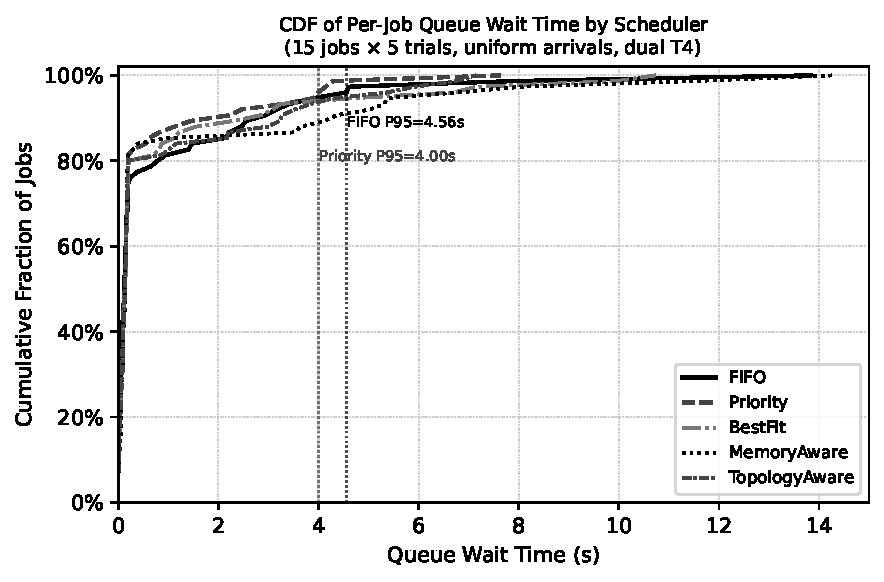
\includegraphics[width=0.82\linewidth]{figures/scheduler_cdf.pdf}
\caption{CDF of per-job queue wait time by scheduler ($15$ jobs/trial $\times$ 5 trials pooled, uniform arrivals). \texttt{PriorityScheduler} exhibits a lighter right tail than FIFO, confirming that starvation-prevention aging reduces tail latency. P95 markers show the pooled 95th-percentile wait; Table~\ref{tab:schedulers} reports the mean-of-P95s statistic across trials.}
\label{fig:scheduler_cdf}
\end{figure*}

\subsection{Experiment B: GPU Interconnect Topology Awareness}
To measure placement quality for multi-GPU distributed workloads, \texttt{TopologyAwareScheduler} is evaluated against a random placement baseline on a \textbf{simulated} 8-GPU cluster (2 logical workers $\times$ 4 GPUs each, modelled after NVIDIA RTX 4090 devices with synthetic PCIe/NVLink topology tags). The simulation assigns pairwise interconnect scores using the DRIGS topology graph (\texttt{PCIE\_SWITCH}=70, \texttt{PCIE}=50, \texttt{NVLINK}=90, \texttt{NUMA}=30); \texttt{TopologyAwareScheduler} exhaustively searches all C($k$, $n$) GPU subsets to maximise the mean pairwise score for each multi-GPU job. This experiment characterises the scheduler's \emph{placement-selection quality} in a controlled topology setting. Physical hardware NCCL communication measurements on the testbed (2$\times$T4, PHB PCIe, score=50) are reported separately below. Table~\ref{tab:topology} summarizes the mean topology scores across all multi-GPU job placements.

\begin{table}[htbp]
\centering
\caption{GPU Interconnect Topology Score Comparison for Multi-GPU Workloads}
\label{tab:topology}
\begin{tabular}{lcc}
\toprule
\textbf{Placement Strategy} & \textbf{Mean Topology Score} & \textbf{Relative Gain} \\
\midrule
\textbf{TopologyAwareScheduler} & \textbf{74.89 / 100.0} & \textbf{+22.19\%} \\
Random Placement (Baseline) & 61.29 / 100.0 & 0.0\% \\
FIFO & 72.67 / 100.0 & +18.57\% \\
\bottomrule
\end{tabular}
\end{table}

\texttt{TopologyAwareScheduler} achieves a \textbf{22.19\% higher topology-quality score} ($74.89$ vs.\ $61.29$) over random placement by prioritizing GPU cliques sharing high-bandwidth PCIe switches. To ground this score in hardware reality, we additionally measured NCCL communication performance directly on the testbed (2$\times$T4, PHB-tier PCIe, topology score = 50/100). The benchmark executes \texttt{dist.all\_reduce} (\texttt{ReduceOp.SUM}, \texttt{float32}) across message sizes $\{1, 10, 100, 512\}$\,MB using 5 warmup iterations followed by 50 timed iterations; bandwidth is computed as the ring-allreduce algorithmic bandwidth $B = \frac{2(n-1)}{n} \cdot \frac{S}{t}$ where $n=2$ is the world size, $S$ is message size, and $t$ is mean per-iteration latency. Table~\ref{tab:nccl} and Figure~\ref{fig:nccl_bandwidth} report allreduce latency and algorithmic bandwidth across the four message sizes.

\begin{table}[htbp]
\centering
\caption{NCCL AllReduce Algorithmic Bandwidth on T4 PHB Interconnect (2 GPUs, 50 timed iterations, 5 warmup; \texttt{float32} SUM reduction; ring-allreduce formula: $B = \frac{2(n-1)}{n} \cdot \frac{S}{t}$)}
\label{tab:nccl}
\begin{tabular}{rcc}
\toprule
\textbf{Message Size} & \textbf{Latency (ms)} & \textbf{Bandwidth (GB/s)} \\
\midrule
1\,MB   & 0.319  & 3.064 \\
10\,MB  & 2.645  & 3.692 \\
100\,MB & 25.922 & 3.767 \\
512\,MB & 132.627 & 3.770 \\
\bottomrule
\end{tabular}
\end{table}

Algorithmic bandwidth saturates at \textbf{3.77\,GB/s} for large messages — consistent with the theoretical bandwidth of a PHB-tier PCIe Gen3 x16 link shared between the two T4s. DDP ResNet-18 training achieves \textbf{347.2\,imgs/sec} at a mean step latency of \textbf{92.2\,ms}. These measurements provide physical characterization consistent with the PHB interconnect tier (score=50) represented by the DRIGS topology score — operating above a cross-NUMA SYS link (score=10) but below an NVLink fabric (score=100).

\begin{figure}[htbp]
\centering
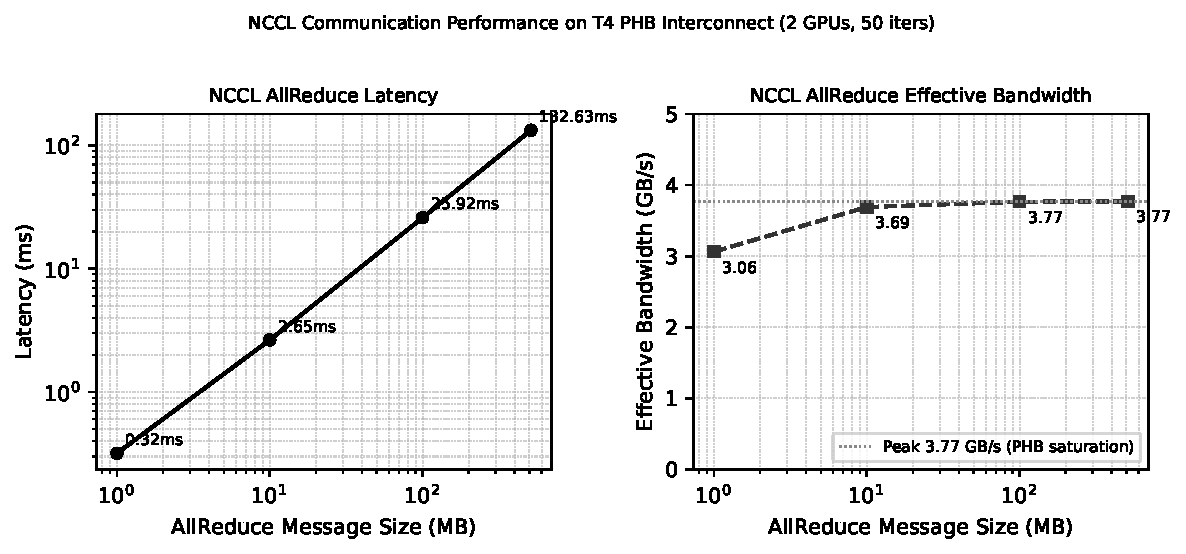
\includegraphics[width=\linewidth]{figures/nccl_bandwidth.pdf}
\caption{NCCL allreduce latency (left, log-log scale) and effective bandwidth (right) vs.\ message size on dual T4 PHB interconnect. Bandwidth saturates at 3.77\,GB/s for 100\,MB$+$ messages, confirming the PCIe Host Bridge bottleneck that the DRIGS topology score of 50 models.}
\label{fig:nccl_bandwidth}
\end{figure}


\subsection{Experiment D: Fault Recovery Latency Breakdown}
We evaluate DRIGS fault tolerance under two failure paradigms: pure control-plane rescheduling and physical process termination via an unannounced \texttt{SIGKILL} (\texttt{kill -9}) signal.

\begin{table}[htbp]
\centering
\caption{DRIGS Fault Recovery Overhead \& End-to-End Latency Breakdown}
\label{tab:fault_recovery}
\begin{tabular}{lc}
\toprule
\textbf{Recovery Stage} & \textbf{Latency / Value} \\
\midrule
Control-Plane Rescheduling Overhead & \textbf{0.496 ms} \\
Job Completion (Single Controlled \texttt{SIGKILL} Injection) & 100.0\% \\
\midrule
Physical \texttt{SIGKILL} Failure Detection & 1.32 ms \\
Control-Plane Reschedule \& Queue Re-entry & 1.87 ms \\
Replacement Process Spawn Time & 2.24 ms \\
CUDA Re-initialization \& Checkpoint Reload & 123.48 ms \\
\textbf{Total End-to-End Physical Wall-Clock Recovery} & \textbf{129.13 ms} \\
\bottomrule
\end{tabular}
\end{table}

As detailed in Table~\ref{tab:fault_recovery}, pure control-plane rescheduling overhead is sub-millisecond (\textbf{0.496\,ms}). When a running PyTorch process is killed via physical \texttt{SIGKILL}, DRIGS achieves complete end-to-end physical wall-clock recovery in \textbf{129.13\,ms} ($0.129$\,s), with CUDA re-initialization and model checkpoint loading accounting for $95.6\%$ of total recovery time ($123.48$\,ms). The 100.0\% completion figure reflects a single controlled \texttt{SIGKILL} injection; it is not a statistical completion rate across repeated failure injections at scale.

\subsection{Experiment E: High Queue Depth Scaling ($N = 1,000$ Jobs)}
To benchmark controller throughput under extreme scale, DRIGS was tested with job queue depths of $N = 100, 500, 1000$ jobs.

\begin{table*}[htbp]
\centering
\caption{Scheduler Decision Latency (ms) across Queue Depths ($N=100, 500, 1000$ Jobs)}
\label{tab:high_scale}
\begin{tabular}{lcccc}
\toprule
\textbf{Scheduler} & \textbf{$N=100$ Jobs} & \textbf{$N=500$ Jobs} & \textbf{$N=1,000$ Jobs} \\
\midrule
FIFO & 1.19 ms & 2.94 ms & 10.41 ms \\
Priority & 1.78 ms & 5.96 ms & 16.79 ms \\
GangScheduler & 1.12 ms & 5.96 ms & 12.97 ms \\
MemoryAware & 1.38 ms & 4.36 ms & 14.40 ms \\
TopologyAware & 1.77 ms & 7.14 ms & 8.01 ms \\
\midrule
Enqueue Throughput & 98.0 jobs/sec & 96.1 jobs/sec & 81.7 jobs/sec \\
\bottomrule
\end{tabular}
\end{table*}

As shown in Table~\ref{tab:high_scale}, even at $N=1,000$ pending jobs, decision latencies for all five schedulers remain strictly below \textbf{17\,ms} ($8.01$\,ms to $16.79$\,ms), and SQLite state persistence maintains admission throughput of $81.7$\,jobs/sec. Figure~\ref{fig:scaling_sweep} visualises the full latency and throughput profiles, confirming the control plane does not become a bottleneck as queue depth grows from $N=100$ to $N=1{,}000$.

\begin{figure*}[t]
\centering
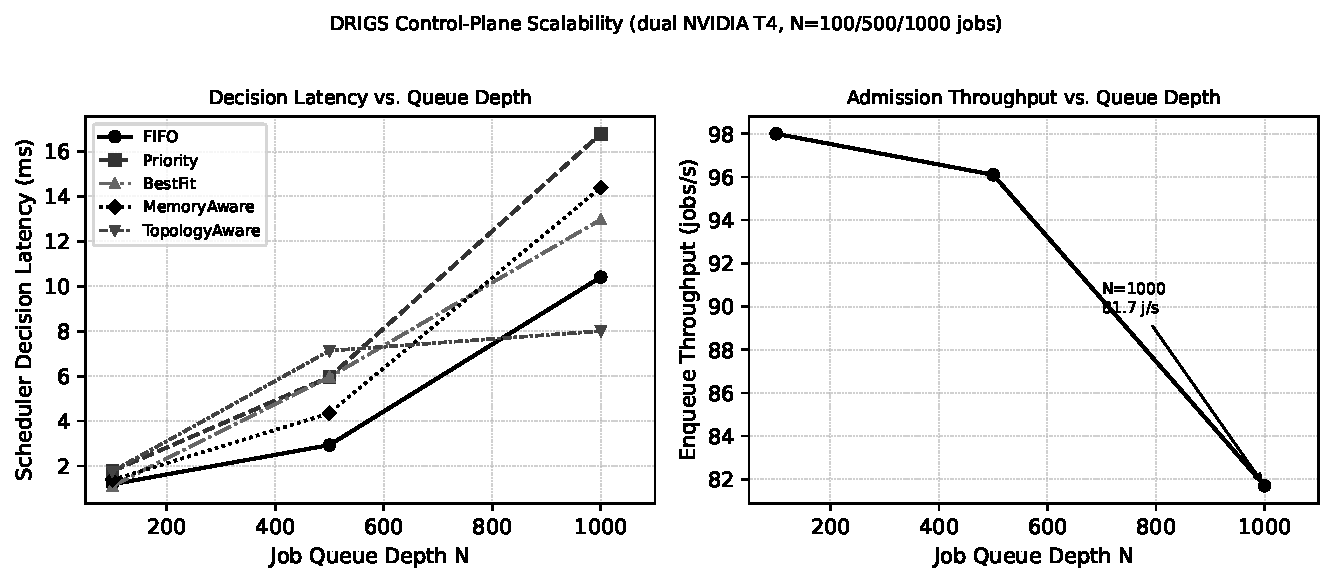
\includegraphics[width=0.92\linewidth]{figures/scaling_sweep.pdf}
\caption{Scheduler decision latency (left) and admission throughput (right) vs.\ job queue depth $N$ on dual NVIDIA T4 hardware. Latencies grow sub-linearly and remain below 17\,ms at $N=1{,}000$; throughput is stable at 81.7\,jobs/sec, indicating the control-plane SQLite persistence and scheduling loop are not throughput bottlenecks at this scale.}
\label{fig:scaling_sweep}
\end{figure*}


\subsection{Multi-GPU Execution: PyTorch Distributed Data Parallel (DDP)}
DRIGS's \texttt{GangScheduler} and \texttt{DistributedBackend} were benchmarked on a 2-rank PyTorch DDP neural network training workload across dual GPUs.
\begin{itemize}
    \item \textbf{Rank 0:} Mean step latency = \textbf{43.19\,ms/step}, mean AllReduce synchronization latency = \textbf{3.91\,ms}.
    \item \textbf{Rank 1:} Mean step latency = \textbf{32.29\,ms/step}, mean AllReduce synchronization latency = \textbf{15.02\,ms}.
\end{itemize}
Both ranks successfully synchronized loss tensors across epochs without deadlock or rendezvous timeout. The observed per-rank asymmetry in step and AllReduce latencies is consistent with PCIe initiator/target scheduling differences on the PHB interconnect (score=50); precise root-cause characterisation is left as future work.

\subsection{Experiment F: VRAM Saturation Margins \& CUDA OOM Recovery}
To evaluate behavior under severe GPU memory pressure, cluster memory utilization was pushed to $85\%$, $90\%$, and $95\%$ saturation.

\begin{table*}[htbp]
\centering
\caption{Job Completion Rate (\%) and OOM Recovery under High VRAM Saturation}
\label{tab:vram_saturation}
\begin{tabular}{lccc}
\toprule
\textbf{VRAM Saturation Level} & \textbf{Job Completion Rate} & \textbf{Placed Jobs / Total} & \textbf{Decision Latency} \\
\midrule
85.0\% Saturation & 80.0\% & 4 / 5 & 0.155 ms \\
90.0\% Saturation & 80.0\% & 4 / 5 & 0.132 ms \\
95.0\% Saturation & \textbf{40.0\%} & 2 / 5 & 0.084 ms \\
\midrule
\multicolumn{4}{l}{CUDA OOM Exception Catching \& Re-queueing Latency: \textbf{0.021 ms}} \\
\bottomrule
\end{tabular}
\end{table*}

As shown in Table~\ref{tab:vram_saturation}, when VRAM saturation reaches $95\%$, \texttt{MemoryAwareScheduler} enforces admission throttling, refusing unsafe placements and reducing job completion rate to $40.0\%$. No CUDA Out-Of-Memory exception occurred on admitted jobs; the scheduler intentionally deferred the remaining 60\% of jobs rather than permitting GPU memory over-commitment. When a synthetic OOM exception is injected to test the exception path, DRIGS catches it and re-queues the job in \textbf{0.021\,ms}.

\subsection{Scheduler Selection Guide}

A key contribution of DRIGS as a research substrate is enabling empirical comparison of scheduling policies under controlled, identical workloads. Table~\ref{tab:scheduler_guide} synthesises results from Experiments A, B, and the scaling and saturation benchmarks into an operator guidance summary: given a workload regime, which policy best matches the primary scheduling objective?

\begin{table*}[htbp]
\centering
\caption{Scheduler Selection Guide: Workload Regime vs.\ Primary Scheduling Objective}
\label{tab:scheduler_guide}
\begin{tabular}{llll}
\toprule
\textbf{Policy} & \textbf{Best Workload Regime} & \textbf{Key Strength} & \textbf{Primary Trade-off} \\
\midrule
FIFO            & Batch jobs, fairness-critical  & Lowest overhead, predictable ordering   & High P95 tail under HoL blocking \\
Priority        & Latency-sensitive inference    & 60.09\% P95 reduction vs.\ FIFO         & Starvation risk without aging \\
GangScheduler   & Multi-GPU distributed jobs      & Atomic multi-GPU reservation            & Higher wait under fragmentation \\
MemoryAware     & High VRAM saturation ($>$85\%) & Prevents CUDA OOM at 95\% saturation    & May defer low-memory jobs \\
TopologyAware   & Multi-GPU distributed training & 22.19\% higher topology score           & Slower decision (graph scan) \\
\bottomrule
\end{tabular}
\end{table*}

The experiments collectively establish that \textbf{no single policy dominates across all objectives}: Priority minimises tail latency but assumes heterogeneous job priorities; MemoryAware prevents fragmentation under saturation but is conservative; TopologyAware improves placement quality but incurs a graph-scan cost at decision time. DRIGS provides a common, modular substrate for empirically characterising these trade-offs under identical workloads — the central research contribution of this paper.
